

\subsection{Fysik teori}

\begin{figure}[H]
\centering
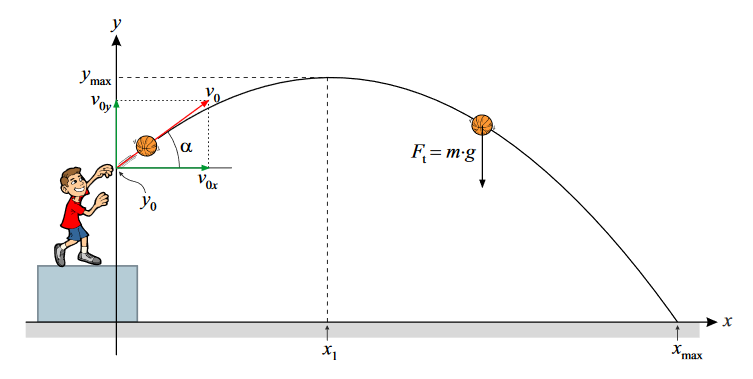
\includegraphics[scale=0.7]{Billeder/skrakast.png}
\caption{Skitse af det skraa kast. Figuren stammer fra \url{http://www.matematikfysik.dk/fys/noter_tillaeg/tillaeg_det_skraa_kast_uden_luftmodstand.pdf}}.
\label{fig:Resultatbehandling3}
\end{figure}

\textbf{Teoretisk udledning af formler til det skrå kast}\\
Begyndelseshastigheden for et kast er givet ud fra vektoren $v_{0}$ og vinklen a, det betyder altså at hastighedsvektorens komposanter kan findes ved:\\

\begin{center}
\begin{math}
\centering
v_{x} = v_{0} \cdot cos(a) \quad \textrm{og} \quad v_{y} = v_{0} \cdot sin(a)
\end{math}
\end{center}

Samtidigt vides det at x- og y-slut kan skrives som to bevægelsesligninger:\\

\begin{center}
\begin{math}
\centering
y = -\dfrac{1}{2} \cdot g \cdot t^{2} + v_{y} \cdot t + y_{0}
\end{math}
\end{center}



Hvor dette er formlen for strækning inden for faget kinematik, omskrevet til at passe på y-aksen i det skrå kast. Her skiftes strækningen ud med y og accelerationen med g, da det er tyngdeaccelerationen som kastet arbejder imod:\\

\begin{center}
\begin{math}
\centering
s = -\dfrac{1}{2} \cdot g \cdot t^{2} + v_{0} \cdot t + s_{0} 
\end{math}
\end{center}

x er derved givet ved konstant hastighed, denne får altså ligningen:\\

\begin{center}
\begin{math}
\centering
x = v_{x} \cdot t
\end{math}
\end{center}

Hvor denne er omskrevet fra formlen for konstant hastighed:\\

\begin{center}
\begin{math}
\centering
v = \dfrac{\Delta s}{\Delta t}
\end{math}
\end{center}




Hvor der isoleres for strækningen:\\

\begin{center}
\begin{math}
v = \dfrac{\Delta s}{\Delta t} \longrightarrow \Delta s = v \cdot \delta t
\end{math}
\end{center}

Dette giver altså to ligninger for x- og y-slut nr komposanterne indsættes:\\

\begin{center}
\begin{math}
x_{slut} = v_{0} \cdot cos(a) \cdot t
\end{math}
\end{center}

og\\

\begin{center}
\begin{math}
y_{slut} = -\dfrac{1}{2} \cdot g \cdot t^{2} + v_{0} \cdot sin(a) \cdot t + y_{0}
\end{math}
\end{center}

\textbf{Bestemmelse af  $x_{slut}$}\\
I vores forsøg kender vi hverken tiden eller $x_{slut}$. Tiden kan dog bestemmes.\\

Det vides at $y_{slut}$ er lig $y_{0}$, da planet forsøget er udført på er ensartet, dette vil altså sige, at både $y_{o}$ og $y_{slut}$ er lig 0. Dette kan altså sættes ind i ligningen for $y_{slut}$ og der kan isoleres for t:\\

\begin{center}
\begin{math}
0 = -\dfrac{1}{2} \cdot g \cdot t^{2} + v_{y} \cdot t + y_{0} \longrightarrow t = \dfrac{v_{y} + \sqrt{2 \cdot g \cdot y_{0} + y^{2}_{y}}}{g}
\end{math}
\end{center}

Den tidligere bestemte y komposant kan indsættes så alle variabler kendes:\\

\begin{center}
\begin{math}
t = \dfrac{v_{0} \cdot sin(a) + \sqrt{2 \cdot g \cdot y_{0} + y^{2}_{y}}}{g}
\end{math}
\end{center}

\textbf{Opsat som vektorfunktion}\\
Vektorfunktioner er givet ud fra en ligning for bevægelsen på x-aksen og bevægelsen på y-aksen:

\begin{center}
\begin{math}
\overrightarrow{r}(t) = 
\begin{pmatrix}
x(t)\\
y(t)
\end{pmatrix}
\end{math}
\end{center}

Da bevægelser er beskrevet ved brug af vektorere opsættes skuddet som en vektorfunktion:

\begin{center}
\begin{math}
\overrightarrow{r}(t) = 
\begin{pmatrix}
v_{0} \cdot cos(a) \cdot t\\
- \dfrac{1}{2} \cdot g \cdot t^{2} + v_{0} \cdot sin(a) \cdot t + y_{0}
\end{pmatrix}
\end{math}
\end{center}

\subsection{Forsøg}
\subsubsection{Apparaturliste}
\begin{itemize}
\item 2x opsætnings stativer
\item 1x BT5 A5 Elektrisk Airsoft Gevær
\item 1x LiDAR af typen Leica “Disto D5”
\item 1x Tomstok
\end{itemize}

\subsubsection{Fremgangsmåde}

\begin{figure}[H]
\centering
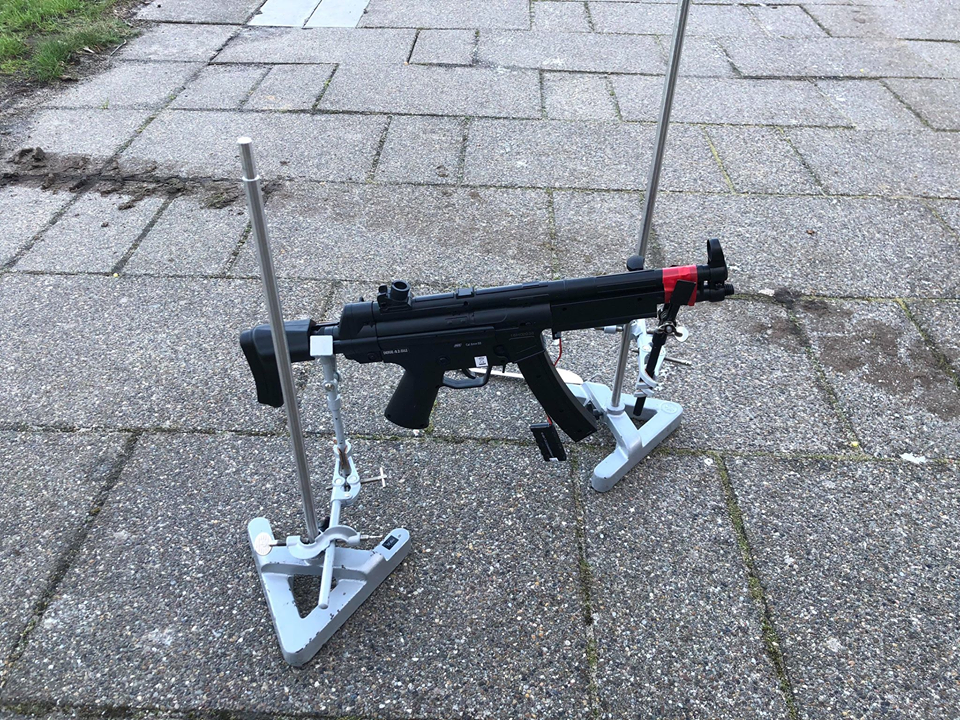
\includegraphics[scale=0.4]{Billeder/Opstilling.png}
\caption{Forsogsopstilling.}
\label{fig:Opstilling}
\end{figure}


\begin{enumerate}
\item Først opsættes det elektriske airsoft gevær på en sådan måde at vinklen er let at ændre, denne opsætning ses på figur \ref{fig:Opstilling}.

\item Der indstilles en vinkel. 
\begin{enumerate}
\item Højden mellem de to monteringspunkter og jorden måles.
\item Der måles en afstand mellem de to monteringspunkter, dette er en hypotenuse mellem de to monteringspunkter.
\item det lave monteringspunkt trækkes fra det høje, og nu er en modstående katete til den ønskede vinkel fundet.
\item Bestem brugt vinkel ud fra sinus beregning.
\end{enumerate}

\item Skud affyres.

\item Afstanden fra skuddets første kontaktpunkt med jorden hen til gevær-opstillingen ved hjælp af LiDAR.

\item Der tages tre målinger for hver vinkel.
\end{enumerate}

\subsubsection{Resultatbehandling}

For at undersøge hypotesen om, hvorvidt det skrå kast er en god model til at beskrive airsoft-geværets skud vil vi sammenligne de teoretiske beregninger med det målte data. Til at gøre dette har vi sammenlignet den teoretisk beregnede $x_{slut}$ med den gennemsnitlige målte $x_{slut}$ ($x_{1}$, $x_{2}$ osv.) for hver vinkel vi har udført målinger med. Den grønne kurve og det sorte punkt er de teoretiske værdier, mens de blå punkter er det målte data.

\begin{figure}[H]
\centering
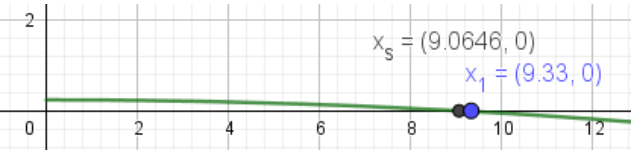
\includegraphics[scale=0.7]{Billeder/Resultatbehandling1.png}
\caption{Korsel 1. Vandret skudvinkel, haevet 0,23 m.}
\label{fig:Resultatbehandling1}
\end{figure}

Som det kan ses på figur \ref{fig:Resultatbehandling1} skyder geværet meget tæt på den teoretiske længde når skudvinklen er vandret. Det betyder at den kendte funktion for det skrå kast uden luftmodstand er en god model til at beskrive skud med denne vinkel, da den ville kunne ramme en skive på størrelse med et menneske, hvis den er indstillet vha. den teoretiske kurve.

\begin{figure}[H]
\centering
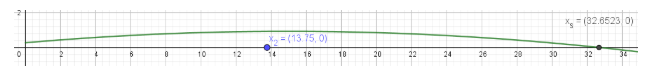
\includegraphics[scale=0.7]{Billeder/Resultatbehandling2.png}
\caption{Korsel 2. Skudvinkel på 5 grader, haevet 0,27 m.}
\label{fig:Resultatbehandling2}
\end{figure}

Som det kan ses på figur \ref{fig:Resultatbehandling2} burde skuddet flyve mere end tredobbelt så langt som før ved denne vinkel, men at dette ikke sker i praksis. For at konstruere en mere beskrivende kurve for skuddet ved 5 grader, kan man modificere kurven for det skrå kast ved at omskrive y(t)-leddet så den hælder dobbelt så meget.

\begin{figure}[H]
\centering
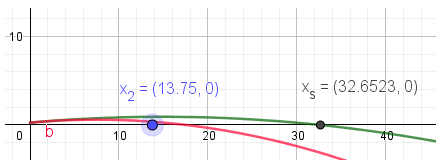
\includegraphics[scale=0.7]{Billeder/Resultatbehandling3.png}
\caption{Korsel 2. Den rode linje angiver den modificerede kurve.}
\label{fig:Resultatbehandling3}
\end{figure}

\begin{center}
\begin{math}
\overrightarrow{r}(t) = 
\begin{pmatrix}
v_{0} \cdot cos(a) \cdot t\\
- \dfrac{1}{2} \cdot g \cdot t^{2} + v_{0} \cdot sin(a) \cdot t + y_{0}
\end{pmatrix}
\end{math}
\end{center}

\begin{center}
\begin{math}
\overrightarrow{r}(t) = 
\begin{pmatrix}
v_{0} \cdot cos(a) \cdot t\\
- \dfrac{1}{2} \cdot g \cdot t^{2} + v_{0} \cdot sin(a) \cdot t + y_{0}
\end{pmatrix}
\end{math}
\end{center}

\begin{center}
\begin{math}
\overrightarrow{r}(t) = 
\begin{pmatrix}
v_{0} \cdot cos(a) \cdot t\\
-1 \cdot g \cdot t^{2} + v_{0} \cdot sin(a) \cdot t + y_{0}
\end{pmatrix}
\end{math}
\end{center}

Som det kan ses på figur \ref{fig:Resultatbehandling3} får kurven en dobbelt så stor hældning ved at multiplikere y(t)-leddet med 2, så $-\dfrac{1}{2}$ bliver til $-1$.

\begin{figure}[H]
\centering
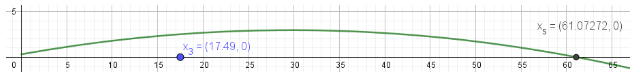
\includegraphics[scale=0.7]{Billeder/Resultatbehandling4.png}
\caption{Korsel 3. Skudvinkel på 10 grader, haevet 0,31 m}
\label{fig:Resultatbehandling4}
\end{figure}

Igen viser figur \ref{fig:Resultatbehandling4} at den teoretiske værdi er mange gange større end den praktiske. Denne gang viser kurven at skuddet burde flyve mere end tredobbelt så langt som tidligere, hvilket peger i retning af at som skudvinklen bliver større, og dermed også længden af skuddets bane, bliver 
den praktiske skudlængde eksponentielt mindre sammenlignet med den teoretiske.\\

Ud fra det kan vi opstille en mere generel kurve til vores skud, som inkorporerer en stigende hældning i takt med at skudvinklen stiger. Dette kan gøres ved at observere, hvordan den teoretiske værdi svinger mere fra den praktiske jo større skudvinklen er. \\

\begin{itemize}
\item For 0 grader:		$x_{teori} = 1x_{praktisk} $
\item For 5 grader:		$x_{teori} = 2x_{praktisk} $
\item For 10 grader:	$x_{teori} = 3x_{praktisk} $
\item For 15 grader:	$x_{teori} = 4x_{praktisk} $
\end{itemize}

Hvis antallet af grader byttes ud med et symbol, kan en generel sammenhæng findes.\\[0.5cm]

For n grader: $ x_{teori} \approx ((\dfrac{n}{5})+1) $\\[0.5cm]

For at opsætte en kurve som følger dette princip, kan vi modificere x(t) så kurvens hældning bliver kraftigere i takt med at skudvinklen stiger.\\

\begin{center}
\begin{math}
x(t) = v_{0} \cdot cos(a) \cdot t
\end{math}
\end{center}

\begin{center}
\begin{math}
x(t) = \dfrac{v_{0} \cdot cos(a) \cdot t}{\dfrac{a}{5} + 1}
\end{math}
\end{center}

\begin{figure}[H]
\centering
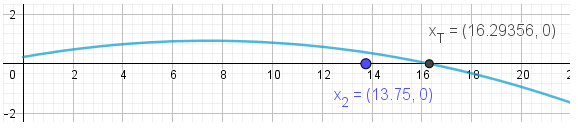
\includegraphics[scale=0.7]{Billeder/Resultatbehandling5.png}
\caption{Den nye funktions slutpunkt sammenlignet med maalepunktet ved 5 grader.}
\label{fig:Resultatbehandling5}
\end{figure}

Som det kan ses på figur \ref{fig:Resultatbehandling5} er der stadig en forskel på ca. 2,5 meter mellem de to nedslagspunkter. Denne forskel kan kraftigt formindskes ved at lægge 1,5 til i stedet for 1 i x(t).\\

\begin{center}
\begin{math}
x(t) = \dfrac{v_{0} \cdot cos(a) \cdot t}{\dfrac{a}{5} + 1.5}
\end{math}
\end{center}

For at undersøge om den nye kurve beskriver skuddene på $ > 5 $ grader mere præcist, kan vi sammenligne dens slutpunkt med målepunkterne. Noter at $ x_{T} $ er det nedslagspunkt kurven forudsiger, hvorimod $x_{2}$, $x_{3}$ etc. er målepunkter.\\

\begin{figure}[H]
\centering
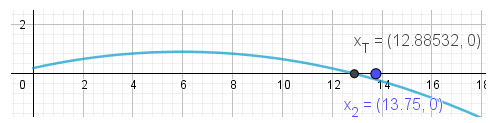
\includegraphics[scale=0.7]{Billeder/Resultatbehandling6.png}
\caption{Den nye kurve og maalepunktet til 5 grader.}
\label{fig:Resultatbehandling6}
\end{figure}

\begin{figure}[H]
\centering
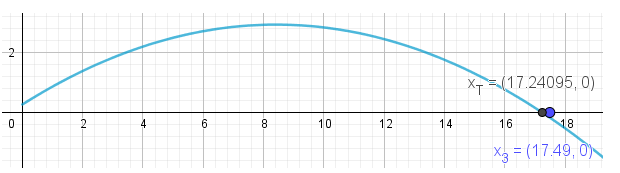
\includegraphics[scale=0.7]{Billeder/Resultatbehandling7.png}
\caption{Den nye kurve og maalepunktet til 10,15 grader.}
\label{fig:Resultatbehandling7}
\end{figure}

\begin{figure}[H]
\centering
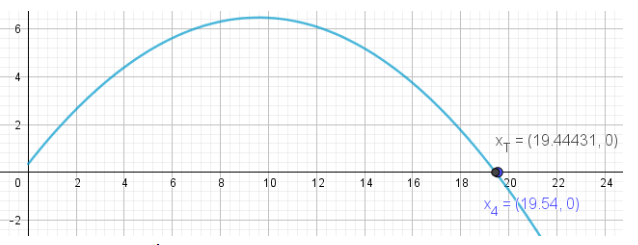
\includegraphics[scale=0.7]{Billeder/Resultatbehandling8.png}
\caption{Den nye kurve og maalepunktet til 15,53 grader.}
\label{fig:Resultatbehandling8}
\end{figure}

Som det kan ses på figur \ref{fig:Resultatbehandling6} , \ref{fig:Resultatbehandling7} og \ref{fig:Resultatbehandling8} passer den nye kurve og dens nedslagspunkt meget præcist på det beregnede. Modellen beskriver altså, hvordan vores airsoft-gevær skyder meget mere præcist end det skrå kast, da denne tager hensyn til vinklen samt konstanten 1,5, der bliver lagt til. Konstanten og hensynet til vinklen bruges altså til at tage luftmodstanden med i beregningen, da denne er forskellen på forsøgsdataet og det skrå kasts teoretiske beregninger.\\[0.5cm]

Kurven til vores airsoft-geværs skud bliver altså beskrevet ved:\\

\begin{center}
\begin{math}
\overrightarrow{r}(t) = 
\begin{pmatrix}
x(t)\\
y(t)
\end{pmatrix}
=
\begin{pmatrix}
\dfrac{v_{0} \cdot cos(a) \cdot t}{\dfrac{a}{5} + 1.5}\\
- \dfrac{1}{2} \cdot g \cdot t^{2} + v_{0} \cdot sin(a) \cdot t + y_{0}
\end{pmatrix}
\end{math}
\end{center}

\newpage
\subsubsection{Diskussion}

Mange faktorer har haft en indflydelse på indsamlingen af måledata til dette forsøg. Først og fremmest var det nødvendigt at lave forsøget udenfor, da geværet både skyder langt og højt. Dette skaber problemer i forhold til vind, da kuglerne er meget lettere. Dette kan blandt andet være grunden til at de længere skud har større variation i hvor de lander, da de har haft længere tid til at blive påvirket af eventuelle vindstød.\\

Samtidigt var det svært at se præcis hvor kuglerne landede da de er små og flyver relativt hurtigt. (Mundingshastigheden er cirka 41 m/s og kuglernes diameter er 6 mm). Dette problem løste vi dog ved at bruge en sandkasse. Her hoppede kuglerne nemlig sjældent efter de ramte jorden og blev som regel liggende hvor de ramte. Dette gjorde selve måle-arbejdet betydeligt meget lettere.\\

Inden vi opsatte vores egen vektorfunktion som model til skuddene, afprøvede vi en anden kendt model for det skrå kast med luftmodstand\footnote{\url{ http://www.matematiksider.dk/projekter/skraakast.pdf}}.\\

\begin{center}
\begin{math}
\overrightarrow{r}(t) = 
\begin{pmatrix}
x(t)\\
y(t)
\end{pmatrix}
=
\begin{pmatrix}
\dfrac{v_{0} \cdot cos(a) \cdot t}{\dfrac{a}{5} + 1.5}\\
- \dfrac{1}{2} \cdot g \cdot t^{2} + v_{0} \cdot sin(a) \cdot t + y_{0}
\end{pmatrix}
\end{math}
\end{center}

Vi fandt dog hurtigt ud af at denne kun er egnet når man arbejder med objekter, der enten er meget tungere eller bevæger sig markant langsommere, da den overestimerer luftmodstanden så meget ved vores skud, at nedslagspunktet ligger indenfor de første 0,5 meter ved alle vinkler.

















